\documentclass{beamer}

\mode<presentation>
{
  \usetheme{Warsaw}
  \setbeamercovered{transparent}
}
\usepackage[english]{babel}
\usepackage[utf8]{inputenc}
\usepackage{times}
\usepackage{float}
\usepackage[T1]{fontenc}

\title[PROYECTO - ANDROID] 
{S E A R C H --- S A V E}


\subtitle{}
\institute[ESCUELA SUPERIOR]
{	
	\centering
  		
\includegraphics[totalheight=1in,width=1in]{ss}
  		
	ESCUELA SUPERIOR\\
	POLITECNICA DEL LITORAL
}
\date[CFP 2012]{Proyecto en Android, 2012}

\begin{document}
	\begin{frame}
  	  \titlepage
	\end{frame}
	
	%Integrantes del Grupo
	\begin {frame}{INTEGRANTES}
		 \begin{flushleft}
 			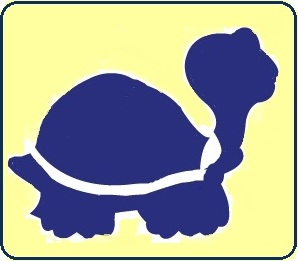
\includegraphics[totalheight=1.2in,width=2in]{LTwitspol}
 		 \end{flushleft}
 		 
 		 \begin{itemize}
 		 	\item
 		 		\begin{flushright}
 		 			Cuadrado Daniel
 		 		\end{flushright}
 		 	\item
 		 		\begin{flushright}
 		 			Mite Juan 
 		 		\end{flushright}
 		 	\item
				\begin{flushright} 		 		
 		 		Torres Criollo Daniel
 		 		\end{flushright}
 		 	\item
 		 		\begin{flushright}
 		 			Velez Gomez José
 		 		\end{flushright}
 		 \end{itemize}
  	\end{frame}
  	  	
  	%Seccion Introduccion
  	\begin{frame}{DESCRIPCION DE LA APLICACION}
  		\centering
  		
\includegraphics[totalheight=1in,width=1in]{ss}	
  		\begin{block}{}
  		La aplicaciónse ejecuta en su mayoría en segundo plano, cuando el usuario ingresa tema de consulta y lo guarda, se ejecuta el navegador y encuentra la primera incidencia de lo buscado y guarda la pagina, la almacena en la micro SD, elimina el tema de consulta de la lista de notas y así vuelve a realizar este proceso hasta que la lista de búsqueda quede vacía.
  		\end{block}				
	\end{frame}
	
	\begin{frame}{FUNCIONALIDADES DE LA APLICACION}
		\centering
  		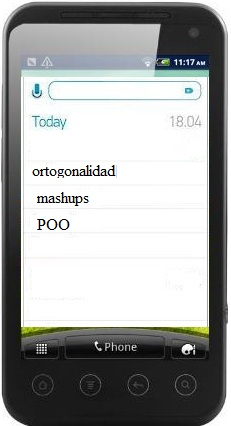
\includegraphics[totalheight=1.4in,width=0.9in]{lt}
  		\begin{block}{}
		La aplicación SEARCH-SAVE resolverá el problema de buscar términos desconocidos por el usuario. La aplicación recibe el tema de consulta, y en segundo plano, ésta se encarga de buscar la información disponible en línea y el usuario la puede revisar cuando quiera.
  		\end{block}				
	\end{frame}
	
  	

\begin{frame}{OBSERVACIONES}
		\centering
  		\begin{block}{}
  		Desarrollar en Android por primera vez requiere de mucha paciencia, tener conocimiento de Java y programación en HTML.
		\end{block}
  		\begin{block}{}
		Tener mucho cuidado con los permisos al buscar un error semántico que no existe en un bloque de código.
  		\end{block}
		\centering
  		\begin{block}{}
  		También revisar el archivo MANIFEST es aquí donde se guarda la estructura esqueleto de la app y donde se deben definir las funcionalidades que se requiere implementar.
  		\end{block}
 	\end{frame}


\begin{frame}{EXPERIENCIAS}
		\centering
  		\begin{block}{}
  		Adquirimos algo de experiencia, ya que era nuestra primera incursión en el desarrollo de aplicaciones Android.
  		\end{block}
		\begin{block}{}
Tuvimos inconvenientes con el IDE y demás cuestiones de instalación.
  		\end{block}
		\begin{block}{}
Fué de gran ayuda el uso de internet, ya que hay muchos soportes, foros, etc.
  		\end{block}
 	\end{frame}

\begin{frame}{CONCLUSIONES}
		\centering
  		\begin{block}{}
		Lo interesante de programar en un lenguaje nuevo para nosotros, significa una especie de reto.
  		\end{block}
  		\begin{block}{}
		El hecho de implementar las funcionalidades suele ser muy complejo.
  		\end{block}
  		\begin{block}{}
		La funcionalidad de nuestra aplicación no era trivial.
  		\end{block}
  		\begin{block}{}
  		Programar en Android es relativamente complicado y mañoso.
  		\end{block}

 	\end{frame}


		
	%\appendix	
	%\section<presentation>*{\appendixname}
	\subsection<presentation>*{SEARCH-SAVE -- ANDROID}
	\begin{frame}
	\centering
		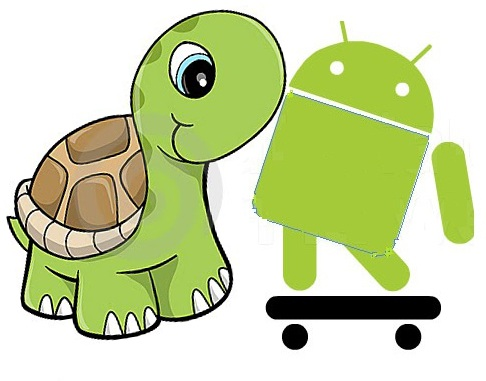
\includegraphics[width=0.3\textwidth]{Android}
		
		\begin{center}
			M U C H A S \\ G R A C I A S 
		\end{center}
	\end{frame}
	
	
\end{document}

